\documentclass[11pt]{beamer}
\usepackage[utf8]{inputenc}
\usepackage[T1]{fontenc}
\usepackage{lmodern}
\usepackage[spanish]{babel}
\usepackage{parskip}
\usepackage{booktabs}
\usepackage{graphicx}
\usetheme{Darmstadt}
\begin{document}
	\author{Mauro Loprete Fabricio Machado}
	\title{El Modelo de la Telaraña}
	\subtitle{Ecuaciones en diferencia de primer orden}
	%\logo{}
	\institute{Cálculo 3}
	\date{9 de septiembre de 2019}
	\subject{Cálculo 3}
	%\setbeamercovered{transparent}
	%\setbeamertemplate{navigation symbols}{}
	\begin{frame}
	\maketitle
	\end{frame}
\begin{frame}
\frametitle{Supuestos}
	$\bullet$ Competencia perfecta
	\\
	$\bullet$ Un único bien
	\\
	$\bullet$ Modelo dinámico
	\\
	$\bullet$ Bien perecedero no almacenable
	\\
	$\bullet$ $Q^s_t$=S($P_{t-1}$) $\quad$ retrasada
	\\	
	$\bullet$ $Q^d_t$=D($P_t$) $\quad$  sin retraso
	\\
	$\bullet$ $Q^s_t$=$Q^d_t$
\end{frame}
\begin{frame}
\frametitle{Condición de equilibrio}
\begin{equation*}
\left\{\begin{matrix}
Q^{s}_{t}=-\gamma+\delta\cdot P_{t-1} \quad (\gamma,\delta >0)
	& \\ Q^{d}_{t}=\alpha-\beta\cdot P_{t}  \quad   (\alpha,\beta>0)
	& \\ Q^{s}_{t}=Q^{d}_{t}
\end{matrix}\right.
\end{equation*}
\\
~
\begin{block}{}
	\begin{center}
		-$\gamma$+$\delta$$P_{t-1}$=$\alpha$-$\beta$$P_t$
	\end{center}
\end{block}
\end{frame}
\begin{frame}
\frametitle{Condición de equilibrio}
	\begin{block}{}
	\begin{center}
			-$\gamma$+$\delta$$P_{t-1}$=$\alpha$-$\beta$$P_t$
	\end{center}
	\end{block}
\begin{center}
\\
$\Longrightarrow$$\delta$$P_{t-1}$+$\beta$+$P_t$=$\alpha$+$\gamma$
\\
$\Longrightarrow$$\delta$$P_t$+$\beta$$P_{t+1}=$$\alpha$$+$$\gamma$ $\quad$ (con t=t+1)
\\
$\Longrightarrow$$\frac{\delta}{\beta}$$P_t$+$P_{t+1}$=$\frac{\alpha+\gamma}{\beta}$
\\
Entonces con c=$\frac{\alpha+\gamma}{\beta}$   a=$\frac{\delta}{\beta}$ tenemos
\\
\begin{block}{}
\begin{center}
	a$P_t$+$P_{t+1}$=c $\space\space\space\space$
\end{center}
\end{block}
\end{center}
\end{frame}
\begin{frame}
\frametitle{Método General}
a$P_t$+$P_{t+1}=c$
\\
$\searrow$ $P_{nh}$:Reducida no homogénea (c$\neq$0) equilibrio intertemporal de p
\\
$\searrow$ $P_{h}$: Reducida homogénea (c=0) desviaciones de las trayectorias de tiempo respecto al equilibrio 
\\
~
\begin{center}
	\begin{block}{Solución general}
	\begin{center}
		$P_t$=Sol$P_h$+una Sol de $P_{nh}$
	\end{center}
	\end{block}
\end{center}
\end{frame}
\begin{frame}
\frametitle{Método General}
Sol$P_h$: a$P_t$+$P_{t+1}$=0
\\
$\Longrightarrow$ a$P_{t-1}$+$P_t$=0 $\quad$ con (t=t-1)
\\
$\Longrightarrow$$P_t$=-a$P_{t-1}$
\\
$\quad$$\searrow$(t=1)$\quad$$P_1$=-a$P_0$
\\
$\quad$$\searrow$(t=2)$\quad$$P_2$=-a$P_1$$\rightarrow$$P_2$=-a(-a$P_0$)
\\
$\quad$$\searrow$(t=3)$\quad$$P_3$=-a$P_2$$\rightarrow$$P_3$=-a(-a.-a.$P_0$)
\\
$\Longrightarrow$$P_t$=-$a^t$$P_0$$\rightarrow$$P_t$=A$b^t$$\quad$con $P_0$=A ya que c=0 y b=-a $\quad$(A$b^t$$\neq$0)
\\
$\Longrightarrow$$P_t$=A$b^t$$\rightarrow$$P_{t+1}$=A$b^{t+1}$$\rightarrow$$P_h$:a(A$b^t$)+A$b^{t+1}$=0$\rightarrow$dividimos por A$b^t$
$\Longrightarrow$a+b=0$\rightarrow$b=-a
\begin{block}{}
\begin{center}
	$P_h$=A$b^t$=A$(-a)^t$
\end{center}
\end{block}
\end{frame}
\begin{frame}
	\frametitle{Método general}
	Sol $P_{nh}$:$\quad$a$P_t$+$P_{t+1}$=c $\quad$ 
	\\
	Asumiendo intertemporalidad (ecuación  en  diferencia  con  término  constante) $P_t$=$P_{t+1}$=k
	\\
	$\Longrightarrow$a(k)+(k)=c$\rightarrow$k(a+1)=c$\rightarrow$k=$\frac{c}{1+a}$$\quad$$\quad$a$\neq$-1 ($\alpha$,$\gamma$>0$\quad$a=$\frac{\delta}{\beta}$)
	\\
	Como $\frac{c}{1+a}$ es una constante, entonces tenemos un equilibrio estacionario
\end{frame}
\begin{frame}
	\frametitle{Método general}
	Sol general($P_t$)=Sol$P_{nh}$+Sol$P_h$=A$(-a)^t$+$\frac{c}{1+a}$$\quad$a$\neq$-1
	\\
	$\Longrightarrow$(t=0)$\quad$$P_0$=A+$\frac{c}{1+a}$$\rightarrow$A=$P_0$-$\frac{c}{1+a}$
	\\
	$P_t$=($P_0$-$\frac{c}{1+a}$)$(-a)^t$+$\frac{c}{1+a}$
	\\
	\begin{equation*}
	P_{t}=(P_{0}-\frac{\frac{\alpha+\gamma}{\beta}}{1+\frac{\delta}{\beta}})(-\frac{\delta}{\beta})^{t}+\frac{\frac{\alpha+\gamma}{\beta}}{1+\frac{\delta}{\beta}}
	\end{equation*}
	\\
\begin{block}{Solución del modelo}
\begin{equation*}
P_{t}=(P_{0}-\frac{\alpha+\gamma}{\beta+\delta})(-\frac{\delta}{\beta})^t+\frac{\alpha+\gamma}{\beta+\delta}
\end{equation*}
\end{block}
\end{frame}
\begin{frame}
\frametitle{Solución particular de la ecuación en diferencia}
\begin{block}{}
	\begin{equation*}
	P_{t}=(P_{0}-\bar{P})((-\frac{\delta}{\beta})^t)+\bar{p}\
\end{equation*}
\end{block}
	$\bar{p}$=$\frac{\alpha+\gamma}{\beta+\delta}$ precio de equilibrio estacionario.
	\\
	~
	Como $\alpha,\beta>0 \quad y \quad b=-a=-\frac{\delta}{\beta}<0$ 
	\\
	\textbf{La solución del modelo es oscilante}
\end{frame}
\begin{frame}
	\frametitle{Tipos de Telarañas}
	\begin{block}{}
		\begin{center}
			$Q^s_t$=-$\gamma$+$\delta$$P_{t-1}$=$\alpha$-$\beta$$P_t$=$Q^d_t$
		\end{center}
	\end{block}
\\
$\delta$ pendiente de $Q^s_t$ y $\beta$ pendiente de $Q^d_t$
\\
\\ $\quad$
\\
\left\{\begin{matrix}
	$\delta$>$\beta$ la oscilación es explosiva
	& \\~ $\delta$<$\beta$ la oscilación es amortiguada
	& \\ $\delta$=$\beta$ la oscilación es uniforme
\end{matrix}
\end{frame}
\begin{frame}
	\frametitle{Desde la óptica del economista}
	Colocamos los precios en el eje de las ordenadas y las cantidades en el eje de las abscisas.
	\\
	Se invierten las relaciones de las pendientes $\delta$ y $\beta$
	\\ $\quad$
	\\
\begin{center}
	\begin{equation*}
\left\{\begin{matrix}
&  & \\ \frac{1}{\beta }> \frac{1}{\delta } \quad Oscilación \quad Amortiguada 
&  & \\ \frac{1}{\delta }< \frac{1}{\beta } \quad Oscilación \quad Explosiva
&  & \\ \beta = \delta \quad Oscilación \quad Uniforme
&  & 
\end{matrix}\right.
\end{equation*}
\end{center}
\end{frame}
\begin{frame}
\frametitle{Aplicación del modelo}
\begin{block}{Solución del modelo}
	\begin{equation*}
	P_{t}=(P_{0}-\frac{\alpha+\gamma}{\beta+\delta})(-\frac{\delta}{\beta})^t+\frac{\alpha+\gamma}{\beta+\delta}
	\end{equation*}
\end{block}
\\
$P_0$=40
\\
$\alpha$=12
\\
$\beta$=0,3
\\
$\gamma$=5
\\
$\delta$=0,25
\\
\begin{block}{}
	\begin{equation*}
		P_t=(40-\frac{12+5}{0.3+0.23})(-\frac{0.25}{0.3})^t+\frac{12+5}{0.3+0.23}
	\end{equation*}
\end{block}
\end{frame}
\begin{frame}
	\frametitle{Valores}
\begin{table}[h]
	\caption{Tabla de Valores}
	\label{tab:my-table}
	\resizebox{\textwidth}{!}{%
		\begin{tabular}{@{}cccc@{}}
			\toprule
			\textbf{Periodo} & \textbf{Cantidad Demandada} & \textbf{Cantidad Ofrecida} & \textbf{Precio en t} \\ \midrule
			0 & 0 & 0 & 40 \\
			1 & 5 & 5 & 23.3 \\
			2 & 0.8 & 0.8 & 37.2 \\
			3 & 4.3 & 4.3 & 25.6 \\
			4 & 1.4 & 1.4 & 35.3 \\
			5 & 3.8 & 3.8 & 27.3 \\
			6 & 1.8 & 1.8 & 34 \\
			7 & 3.5 & 3.5 & 28.4 \\
			8 & 2.1 & 2.1 & 33 \\
			9 & 3.3 & 3.3 & 29.1 \\
			10 & 2.3 & 2.3 & 32.4 \\\bottomrule
		\end{tabular}%
	}
\end{table}
\end{frame}
\begin{frame}
	\frametitle{Aplicación del modelo a problemas de economía laboral}
	$\bullet$ Mercado de profesionales con elevada formación
	\\
	$\bullet$ Rigideces en la oferta laboral
	\\
	$\bullet$ Oscilación amortiguada
\end{frame}
\begin{frame}{Ejemplo}
	El advenimiento de un pandemia aumentó la demanda de virólogos en el mercado laboral. Se produce por tanto un exceso de demanda que permite a los profesionales ya formados obtener mayores salarios. Esta información llega al mercado laboral pero no logra la entrada inmediata de trabajadores a este sector ya que requieren de un período de formación (t). 
	Pasados t años ingresarán los nuevos virólogos al mercado laboral generando un exceso de oferta que reducirá el salario, enviando información a los nuevos estudiantes que optarán por carreras mejor remuneradas generando una nueva escasez que subirá el salario, y así sucesivamente hasta llegar al equilibrio.
\end{frame}
\begin{frame}
	\begin{center}
		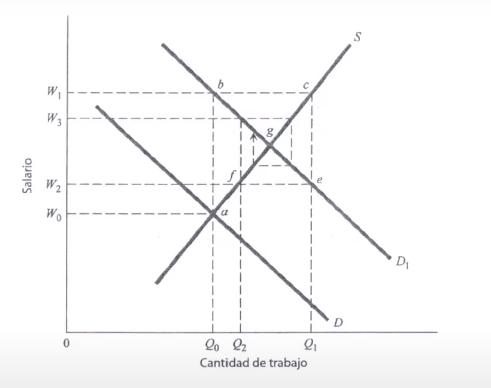
\includegraphics[scale = 0.8]{2.png}
	\end{center}
\end{frame}
\begin{frame}{Criticas a la aplicación del modelo para este problema}
	Las críticas van dirigidas a las variaciones bruscas de la oferta laboral. Entre los postulados que pueden poner en duda ese comportamiento se encuentran, la toma de decisiones mediante un análisis intertemporal, y el hecho de que los individuos pueden tener en cuenta los posibles cambios dentro del mercado laboral y por tanto generarán expectativas racionales sobre las consecuencias de dichas variaciones. Si se cumple alguno de estos postulados se puede llegar al equilibrio sin pasar por la telaraña.
	\footnote{$\tiny$Ejemplo extraído de McConnell C. R., Brue S. L., Macpherson, D. A. (2007)}
\end{frame}
\end{document}